\section{Introduction}

Differentiable programming has a rich history among dynamic languages like Python, Lua and JavaScript, with early implementations including projects like Theano, Torch, and TensorFlow. More recently, their innovations have spread into statically typed, functional languages, such as Haskell (e.g. Stalin$\nabla$ \cite{c1}), F\# (e.g. DiffSharp \cite{c2}) and Swift \cite{c10}. However the majority of existing automatic differentiation (AD) frameworks require the use of an embedded DSL, and comparatively few offer native support in a general-purpose, statically typed programming language.

Prior AD implementations for the JVM include COJAC \cite{c6}, ADiJaC \cite{c7} and DeepLearning4j \cite{c8}, however these implementations either (1) rely on a custom compiler toolchain, (2) are limited to a fixed computation graph, or (3) are intended for a domain specific audience. In contrast, our approach can be applied to native Kotlin, is not tied to the JVM and supports a broad set of use cases, enabling a greater degree of safety, flexibility and expressiveness.

To our present knowledge, Kotlin has no native AD implementation. However, the langauge does contain a number of desirable features for implementing such a framework. As a strong, statically-typed language, we aim to make full use of those capabilities. In addition to Kotlin's type safety and multi-platform support, Kotlin$\nabla$ relies on three language features for maximum effect:

\begin{enumerate}
  \item \textbf{Operator overloading} enables a concise notation for arithmetic on algebraic structures, i.e. group, rings, and fields.
  \item \textbf{Lambdas and coroutines} supports functions as first-class citizens and shift-reset continuations for pure functional AD.
  \item \textbf{Extension functions} allows extending types with new fields and methods without requiring sub-classing or inheritance.
\end{enumerate}

For the purposes of automatic differentiation, we are mostly interested in algebraic fields. By encoding properties of fields in a hierarchy of generically-typed interfaces, we are able to construct a rich grammar by composing the operations of addition, multiplication and division. We believe these algebraically-grounded abstractions will reduce code duplication and help users reason more carefully about differentiable programs to avoid many classes of runtime errors. By carefully designing the API to utilize type inference, these abstractions are mostly invisible to the user.

\section{Usage}
% \begin{minted}
% {kotlin}
% import edu.umontreal.kotlingrad.calculus.DoublePrecision

% with(DoublePrecision) {   //  Double precision  numerics
%   val x = variable("x") //  Define immutable variables
%   val y = variable("y") //  that take numerical values

%   //  Write down a symbolic expression to be evaluated
%   val z = x * (-sin(x * y) + y)      // Infix notation
  
%   // Lazily compute reverse-mode automatic derivatives
%   val dz_dx = d(z) / d(x)          // Leibniz notation
%   val dz_dy = d(z) / d(y)       // Partial derivatives
%   val d2z_dx2 = d(dz_dx) / d(x)  // Higher derivatives
%   val d2z_dxdy = d(dz_dx) / d(y)    // Higher partials
%   val grad_z = z.grad()           // Gradient operator

%   //  Now, we bind values to each independent variable
%   //  and invoke the derivative functions to calculate
%   //  an exact numerical gradient from each expression
%   println(dz_dx(x to 0, y to 1))       // [    1.0   ]
%   println(dz_dy(x to 0, y to 1))       // [    0.0   ]
%   println(d2_dx2(x to 0, y to 1))      // [   -2.0   ]
%   println(d2z_dxdy(x to 0, y to 1))    // [    1.0   ]
%   println(grad_z(x to 0, y to 1))      // [ 1.0, 0.0 ]
% }
% \end{minted}

\begin{figure}[!htb]
\begin{minted}
{kotlin}
import edu.umontreal.kotlingrad.calculus.DoublePrecision

with(DoublePrecision) { // Use double-precision numerics
  val x = variable()  // Declare an immutable variable
  val y = sin(sin(sin(x)))/x + sin(x) * x + cos(x) + x
  
  // Lazily compute reverse-mode automatic derivatives
  val dy_dx = d(y) / d(x)
  val d2y_dx = d(dy_dx) / d(x)
  val d3y_dx = d(d2y_dx2) / d(x)
  val d4y_dx = d(d3y_dx3) / d(x)
  val d5y_dx = d(d4y_dx4) / d(x)

  plot(-10..10, dy_dx, dy2_dx, d3y_dx, d4y_dx, d5y_dx)
}
\end{minted}
\caption{Kotlin$\nabla$ program with one independent variable.}
\label{label:fig1}
\end{figure}

\begin{figure}[!htb]
\textbf{Higher-order derivatives of the function}
\par\medskip
$y = \frac{\sin{\sin{\sin{x}}}}{x} + x * \sin{x} + \cos{x} + x$
\par\medskip
\includegraphics[scale=0.48]{plot.png}
\caption{Output generated by the program shown in Fig. \ref{label:fig1}.}
\end{figure}

\section{DESIGN}

Key to the design of Kotlin$\nabla$ is the notion of \textit{mathematical context} and \textit{operator overloading}. A context is simply a numerical format in which to perform computation. When the user first defines a variable inside a context, that variable and everything the variable comes into contact with will become part of the Kotlin$\nabla$ computation graph. Variables are the entrypoint for all subsequent operations which can be performed. There are three ways to define a computation graph:

\begin{itemize}
    \item \texttt{val z = (x + y) * (x * y)}
    \item \texttt{val z = (x.plus(y)).times(y.times(x))}
    \item \texttt{val z = times(plus(x, y), times(x, y))}
\end{itemize}

While the first form is preferred, all three of these are equivalent ways to construct the same symbolic expression. It should be noted that this expression by itself does not perform any computation - it simply constructs a DAG of function compositions which can be assigned to a variable and invoked lazily at a later point in execution.

We can envision the AST for the expression in Fig. \ref{label:fig1} as follows:

\begin{figure}[!htb]
\textbf{An abstract syntax tree (AST) for the expression}
\par\medskip
\begin{minted}
{kotlin}
val y = sin(sin(sin(x))) / x + sin(x) * x + cos(x) + x
\end{minted}
\par\medskip
\centering
\begin{tikzpicture}[scale=1.1]
\Tree [.+ \texttt{\textbf{x}} [.+ [.\texttt{cos} \texttt{\textbf{x}} ] [.+ [.$\times$ \texttt{\textbf{x}} [.\texttt{sin} \texttt{\textbf{x}} ] ] [.$\div$ [.\texttt{sin} [.\texttt{sin} [.\texttt{sin} \texttt{\textbf{x}} ] ] ] \texttt{\textbf{x}} ] ] ] ]
\end{tikzpicture}
\caption{Implicit AST using function composition}
\end{figure}

Since the expression is also a function, invoking this expression with a particularly value will return a value. We can pass a value to it and print the result like so:

\begin{minted}
{kotlin}
println(y(1)) // Prints "3.06020376804..."
\end{minted}

Similarly, for any of the derivatives calculated in Fig. \ref{label:fig1}:

\begin{minted}
{kotlin}
println(dy_dx(1)) // Prints "1.12638009890..."
\end{minted}

\section{WORK IN PROGRESS}

Kotlin$\nabla$ is a new form AD using algebraic types that also borrows heavily from prior work in functional \cite{c1}, type-safe \cite{c2} differentiable programming \cite{c5}. Through a combination of JVM bytecode and source code analysis, we are able to partially recover symbolic expressions for the gradient as in \cite{c6}. Adapting from Breuleux et al. \cite{c4}, we can perform reverse-mode AD on an abstract syntax tree (AST). And applying Elliot's framework of generalized linear maps \cite{c3} to Kotlin's type system, we can support shape-inference and make simple variable substitutions.

While this project is currently still in its infancy, our goal is to utilize Kotlin's compiler plugin framework and existing multiplatform infrastructure to implement truly native, differentiable programming in a type-safe environment. This will allow users to perform gradient-based computation using a single codebase on multiple architectures and platforms, while leveraging the existing tools and libraries from the JVM ecosystem.

\bibliography{sample}

\begin{thebibliography}{99}

\bibitem{c1} Barak A. Pearlmutter and Jeffrey Mark Siskind, Reverse-Mode AD in a functional framework: Lambda the ultimate backpropagator. TOPLAS 30(2):1-36, Mar 2008, doi:10.1145/1330017.1330018.

\bibitem{c2} Atilim G{\"{u}}nes Baydin, Barak A. Pearlmutter, Alexey Andreyevich Radul, Jeffrey Mark Siskind (2015) Automatic differentiation and machine learning: a survey. arXiv preprint. arXiv:1502.05767

\bibitem{c3} Conal Elliott. The Simple Essence of Automatic Differentiation. Proc. ACM Program. Lang., 2(ICFP):70:1-70:29, July 2018.

\bibitem{c4} Olivier Breuleux and Bart van Merri\"enboer.  Automatic differentiation in Myia. In NIPS AutoDiff Workshop, 2017.

\bibitem{c5} Fei Wang, Xilun Wu, Gregory  Essertel, James Decker, and Tiark Rompf. Demystifying Differentiable Programming:  Shift/Reset the Penultimate Backpropagator.

\bibitem{c6} Monnard, Romain. COJAC Enriched Numbers. Diss. 2014.

\bibitem{c7} Slusanschi, Emil \& Dumitrel, Vlad. (2016). ADiJaC -- Automatic Differentiation of Java Classfiles. ACM Transactions on Mathematical Software. 43. 1-33.

\bibitem{c8} Eclipse Deeplearning4j Development Team. Deeplearning4j: Open-source distributed deep learning for the JVM. http://deeplearning4j.org

\bibitem{c9}  George, M.D. jAlgebra, An abstract algebra library for Java. GitHub repository. \url{https://github.com/mdgeorge4153/jalgebra}

\bibitem{c10}  Wei, Richard. First-Class Automatic Differentiation in Swift: A Manifesto. Gist. \url{https://gist.github.com/rxwei/30ba75ce092ab3b0dce4bde1fc2c9f1d}

\end{thebibliography}